%%%%%%%%%%%%%%%%%%%%%%%%%%%%%%%%%%%%%%%%%%%%%%%%%%%
%
%  New template code for TAMU Theses and Dissertations starting Fall 2012.  
%  For more info about this template or the 
%  TAMU LaTeX User's Group, see http://www.howdy.me/.
%
%  Author: Wendy Lynn Turner 
%
%%%%%%%%%%%%%%%%%%%%%%%%%%%%%%%%%%%%%%%%%%%%%%%%%%%

\documentclass[12pt]{report}
\usepackage[letterpaper]{geometry}
\geometry{verbose,tmargin=1.25in,bmargin=1.25in,lmargin=1.4in,rmargin=1.15in}
 \usepackage[doublespacing]{setspace}
 \usepackage{tocloft}
 \usepackage[rm, tiny,center, compact]{titlesec}
 \usepackage{indentfirst}
 \usepackage{etoolbox}
\usepackage{tocvsec2}
 \usepackage[titletoc]{appendix}
 \usepackage{appendix}
 \usepackage{tamuconfig}
\usepackage{rotating}

% Added to fix issues with pdf searching in some versions of LaTeX
%\usepackage[T1]{fontenc}\usepackage{lmodern}
%%%%%%%%%%%%%%%%%%%%%%%%%%%%%

% Hyperref setup below.  You should be able to get away with using uncommenting just the first line.
%\usepackage[hidelinks]{hyperref}

% if \usepackage[hidelinks]{hyperref} doesn't work try this.
% \usepackage{hyperref}  % Hidelinks is an option that removes link visiability.  TAMU Thesis Offices prefers to not see the links. But often doesn't work.  
% 
% \hypersetup{
%     colorlinks=true,
%     linkcolor=black,
%     citecolor=black,
%     filecolor=black,
%     urlcolor=black,
% }
%%%%%%%  End of hyperref setup.  One of these two options should work, but my motto with hyperref is when in doubt, comment it out!
%%%%%%%%%  This hopefully fixes the problem with vertical spacing of section headings at the top of the page..  Commented out in 1.0.7
% \preto\section{%
% \ifnum\value{section}>0\addtocontents{toc}{\vskip-6pt}\fi
% }
% \preto\subsection{%
% \ifnum\value{subsection}=0\addtocontents{toc}{\vskip-6pt}\fi
% \ifnum\value{subsection}>0\addtocontents{toc}{\vskip-6pt}\fi
% } 
%%%%%%%%%%%%%%%%%%%%%%%%%%%%%%%%%%%%%%%%%%%%%%%%%%%%%%

\begin{document}

\renewcommand{\tamumanuscripttitle}{Active remote setpoint optimization utilizing BAS trend data}
\renewcommand{\tamupapertype}{Dissertation}
\renewcommand{\tamufullname}{Mitchell Thomas Paulus}
\renewcommand{\tamudegree}{Doctor of Philosophy}
\renewcommand{\tamuchairone}{Dr. David Claridge}
% Uncomment out the next line if you have co-chairs.  You will also need to edit the titlepage.tex file.
%\newcommand{\tamuchairtwo}{Additional Chair Name}
\renewcommand{\tamumemberone}{Dr. Charles Culp}
\newcommand{\tamumembertwo}{Dr. Bryan Rasmussen}
\newcommand{\tamumemberthree}{Dr. Juan-Carlos Baltazar}
\renewcommand{\tamudepthead}{Head of Department}
\renewcommand{\tamugradmonth}{May}
\renewcommand{\tamugradyear}{2016}
\renewcommand{\tamudepartment}{Mechanical Engineering}


%%%%%%%%%%%%%%%%%%%%%%%%%%%%%%%%%%%%%%%%%%%%%%%%%%%
%
%  New template code for TAMU Theses and Dissertations starting Fall 2012.  
%  For more info about this template or the 
%  TAMU LaTeX User's Group, see http://www.howdy.me/.
%
%  Author: Wendy Lynn Turner 
%	 Version 1.0 
%  Last updated 8/5/2012
%
%%%%%%%%%%%%%%%%%%%%%%%%%%%%%%%%%%%%%%%%%%%%%%%%%%%

%%%%%%%%%%%%%%%%%%%%%%%%%%%%%% 
%% TITLE PAGE
%% The values get updated automatically.  Please do not make changes to this file other than adding/deleting committee members where necessary.
%%%%%%%%%%%%%%%%%%%%%%%%%%%%%%

\providecommand{\tabularnewline}{\\}



\begin{titlepage}
\begin{center}
\MakeUppercase{\tamumanuscripttitle}
\vspace{4em}

A \tamupapertype

by

\MakeUppercase{\tamufullname}

\vspace{4em}

\begin{singlespace}

Submitted to the Office of Graduate and Professional Studies of \\
Texas A\&M University \\

in partial fulfillment of the requirements for the degree of \\
\end{singlespace}

\MakeUppercase{\tamudegree}
\par\end{center}
\vspace{2em}
\begin{singlespace}
\begin{tabular}{ll}
 & \tabularnewline
& \cr
% If you have Co-Chairs comment out the 'Chair of Committee' line below and uncomment the 'Co-Chairs of Committee' line.
Chair of Committee, & \tamuchairone\tabularnewline
%Co-Chairs of Committee, & \tamuchairone\tabularnewline & \tamuchairtwo\tabularnewline
Committee Members, & \tamumemberone\tabularnewline
 & \tamumembertwo\tabularnewline
 & \tamumemberthree\tabularnewline
Head of Department, & \tamudepthead\tabularnewline

\end{tabular}
\end{singlespace}
\vspace{3em}

\begin{center}
\tamugradmonth \hspace{2pt} \tamugradyear

\vspace{3em}

Major Subject: \tamudepartment \par
\vspace{3em}
Copyright \tamugradyear \hspace{.5em}\tamufullname 
\par\end{center}
\end{titlepage}
\pagebreak{} % This is simply a file that formats and adds your titlepage, please do not edit this unless you have a specific need. .
%%%%%%%%%%%%%%%%%%%%%%%%%%%%%%%%%%%%%%%%%%%%%%%%%%%
%
%  New template code for TAMU Theses and Dissertations starting Fall 2012.  
%  For more info about this template or the 
%  TAMU LaTeX User's Group, see http://www.howdy.me/.
%
%  Author: Wendy Lynn Turner 
%	 Version 1.0 
%  Last updated 8/5/2012
%
%%%%%%%%%%%%%%%%%%%%%%%%%%%%%%%%%%%%%%%%%%%%%%%%%%%
%%%%%%%%%%%%%%%%%%%%%%%%%%%%%%%%%%%%%%%%%%%%%%%%%%%%%%%%%%%%%%%%%%%%%
%%                           ABSTRACT 
%%%%%%%%%%%%%%%%%%%%%%%%%%%%%%%%%%%%%%%%%%%%%%%%%%%%%%%%%%%%%%%%%%%%%

\chapter*{\texorpdfstring{\MakeUppercase{ABSTRACT}}{ABSTRACT}}
\addcontentsline{toc}{chapter}{ABSTRACT} % Needs to be set to part, so the TOC doesnt add 'CHAPTER ' prefix in the TOC.

\pagestyle{plain} % No headers, just page numbers
\pagenumbering{roman} % Roman numerals
\setcounter{page}{2}

\indent  In this work, a new concept was explored for the optimization
of heating, ventilating, and air-conditioning (HVAC) systems in
buildings. The methods assume that only commonly trended sensor data
would be available and that no live connection to trend values would
exist.  An actual implementation would only require a small script to be
written at the target building to request information from a centralized
server and update setpoint values. 

A prioritization of sensors to trend at buildings is presented.
Investigations into the feasibility were completed on a case study
building on the Texas A\&M Campus, the National Center for Therapeutic
Medicine (NCTM). The algorithms and models for the optimization are
presented, along with uncertainty analysis into several key model
parameters. 

Approximately 23-29\% energy savings were found for AHU-2-3 at the NCTM
building from June 1\textsuperscript{st}, 2016 to January
1\textsuperscript{st}, 2017.  Missing fan power and air flow sensors
reduced effectiveness, along with uncertainty in the plenum temperature
for the series fan powered terminal units. Lack of readily available,
accurate, manufacturers specifications were also limitations.  

A prototype of the backend system was developed on the web application
\textit{CC-Compass}, available at Texas A\&M. The system was set up with
a parent-child hierarchy for equipment and equipment properties are
specified in a JSON format. 
 

\pagebreak{}

%%%%%%%%%%%%%%%%%%%%%%%%%%%%%%%%%%%%%%%%%%%%%%%%%%%
%
%  New template code for TAMU Theses and Dissertations starting Fall 2012.  
%  For more info about this template or the 
%  TAMU LaTeX User's Group, see http://www.howdy.me/.
%
%  Author: Wendy Lynn Turner 
%	 Version 1.0 
%  Last updated 8/5/2012
%
%%%%%%%%%%%%%%%%%%%%%%%%%%%%%%%%%%%%%%%%%%%%%%%%%%%

%%%%%%%%%%%%%%%%%%%%%%%%%%%%%%%%%%%%%%%%%%%%%%%%%%%%%%%%%%%%%%%%%%%%%%
%%                           DEDICATION
%%%%%%%%%%%%%%%%%%%%%%%%%%%%%%%%%%%%%%%%%%%%%%%%%%%%%%%%%%%%%%%%%%%%%
\chapter*{\texorpdfstring{\MakeUppercase{DEDICATION}}{DEDICATION}}
\addcontentsline{toc}{chapter}{DEDICATION}  % Needs to be set to part, so the TOC doesnt add 'CHAPTER ' prefix in the TOC.

%% To my family - Mom, Dad, Joe, and Val and to all those who have made the entire experience worthwhile.

To those relentlessly making this world a better place...


\pagebreak{}

%%%%%%%%%%%%%%%%%%%%%%%%%%%%%%%%%%%%%%%%%%%%%%%%%%%
%
%  New template code for TAMU Theses and Dissertations starting Fall 2012.  
%  For more info about this template or the 
%  TAMU LaTeX User's Group, see http://www.howdy.me/.
%
%  Author: Wendy Lynn Turner 
%	 Version 1.0 
%  Last updated 8/5/2012
%
%%%%%%%%%%%%%%%%%%%%%%%%%%%%%%%%%%%%%%%%%%%%%%%%%%%


%%%%%%%%%%%%%%%%%%%%%%%%%%%%%%%%%%%%%%%%%%%%%%%%%%%%%%%%%%%%%%%%%%%%%%
%%                           ACKNOWLEDGEMENTS
%%%%%%%%%%%%%%%%%%%%%%%%%%%%%%%%%%%%%%%%%%%%%%%%%%%%%%%%%%%%%%%%%%%%%
\chapter*{\texorpdfstring{\MakeUppercase{ACKNOWLEDGEMENTS}}{ACKNOWLEDGEMENTS}}
\addcontentsline{toc}{chapter}{ACKNOWLEDGEMENTS}  % Needs to be set to part, so the TOC doesnt add 'CHAPTER ' prefix in the TOC.


%There are certainly too many people to thanks with regards to this work. I would like to thank Dr. Claridge for his support throughout the entire process, trusting that the idea would eventually pan out.

To be filled.

\pagebreak{}

%%%%%%%%%%%%%%%%%%%%%%%%%%%%%%%%%%%%%%%%%%%%%%%%%%%
%
%  New template code for TAMU Theses and Dissertations starting Fall 2012.  
%  For more info about this template or the 
%  TAMU LaTeX User's Group, see http://www.howdy.me/.
%
%  Author: Wendy Lynn Turner 
%	 Version 1.0 
%  Last updated 8/5/2012
%
%%%%%%%%%%%%%%%%%%%%%%%%%%%%%%%%%%%%%%%%%%%%%%%%%%%

%%%%%%%%%%%%%%%%%%%%%%%%%%%%%%%%%%%%%%%%%%%%%%%%%%%%%%%%%%%%%%%%%%%%%%
%%                           NOMENCLATURE
%%%%%%%%%%%%%%%%%%%%%%%%%%%%%%%%%%%%%%%%%%%%%%%%%%%%%%%%%%%%%%%%%%%%%

\chapter*{\texorpdfstring{\MakeUppercase{NOMENCLATURE}}{NOMENCLATURE}}
\addcontentsline{toc}{chapter}{NOMENCLATURE}  % Needs to be set to part, so the TOC doesnt add 'CHAPTER ' prefix in the TOC.

\noindent
\begin{longtable}{ll}
AHU          & Air Handling Unit\tabularnewline
ANN          & Artificial Neural Network                                 \\
API          & Application Program Interface                             \\
ARMA         & Autoregressive-Moving Average                             \\
BAS          & Building Automation System\tabularnewline
CAV          & Constant Air Volume                                       \\
CCLT         & Cooling Coil Leaving Temperature                          \\
CFM          & Cubic Feet per Minute                                     \\
CHW          & Chilled Water                                             \\
COP          & Coefficient of Performance                                \\
CV           & Coefficient of Variation                                  \\
DAT          & Discharge Air Temperature                                 \\
DDC          & Direct Digital Control                                    \\
DX           & Direct Expansion                                          \\
EIB          & European Installation Bus                                 \\
FFLP         & Fraction of Full Load Power                               \\
FPVAV        & Fan Powered Variable Air Volume                           \\
FSM          & Finite State Machine                                      \\
HP           & Horsepower                                                \\
HTTP         & Hypertext Transfer Protocol                               \\
HVAC         & Heating, Ventilation, and Air-Conditioning\tabularnewline
IAQ          & Indoor Air Quality                                        \\
JSON         & JavaScript Object Notation                                \\
MPC          & Model Predictive Control                                  \\
NCTM         & National Center for Therapeutics Manufacturing            \\
NOAA         & National Oceanic and Atmospheric Administration           \\
OA           & Outdoor Air                                               \\
OAHU         & Outdoor Air Handling Unit                                 \\
PID          & Proportional-Integral-Derivative                          \\
PLR          & Part Load Ratio                                           \\
RA           & Return Air                                                \\
RH           & Relative Humidity                                         \\
RMSE         & Root Mean Squared Error                                   \\
RT           & Return Temperature                                        \\
S/S          & Start/Stop                                                \\
SA           & Supply Air (from AHU)                                     \\
VAV          & Variable Air Volume                                       \\
XML          & eXtensible Markup Language                                \\
\(\delta\)   & Uncertainty                                               \\
\(\rho\)     & Density                                                   \\
\(A\)        & Constant for Fraction of Full Load Power                  \\
\(c_{p}\)    & Specific Heat                                             \\
\(\dot{E}\)  & Power                                                     \\
\(h_{v}\)    & Latent Heat of Vaporization                               \\
\( \dot{Q}\) & Heat Load                                                 \\
\(\Delta P\) & Change in Pressure                                        \\
\(t\)        & Time\tabularnewline
\(T\)        & Temperature\tabularnewline
\(\dot{V}\) & Volume Flow Rate                                                                  \\
\(\dot{W}\) & Power                                                                             \\
\(X\)       & Fraction                                                                          \\
\(C_{air}\) & \parbox[t]{5in}{Volumetric Heat Capacity [Energy per unit Volume per unit Temperature Difference] } \\
\(H\)       & Volumetric Heat of Vaporization [Energy per unit Volume]                          \\
\end{longtable}


\vspace{2em}

\noindent
Subscripts

\noindent
\begin{tabular}{ll}
    a    & air                                    \\
    db   & dry-bulb                               \\
    des  & design                                 \\
    dis  & discharge (from terminal unit to zone) \\
    ma   & mixed air                              \\
    oa   & outdoor air                            \\
    plen & plenum                                 \\
    pri  & primary                                \\
    ra   & return air                             \\
    sa   & supply air (from AHU)                  \\
    tot  & total                                  \\
    z    & zone                                   \\
\end{tabular}


\pagebreak{}


%%%%%%%%%%%%%%%%%%%%%%%%%%%%%%%%%%%%%%%%%%%%%%%%%%%
%
%  New template code for TAMU Theses and Dissertations starting Fall 2016.  
%
%
%  Author: Sean Zachary Roberson
%  Version 3.17.09
%  Last Updated: 9/21/2017
%
%%%%%%%%%%%%%%%%%%%%%%%%%%%%%%%%%%%%%%%%%%%%%%%%%%%
%%%%%%%%%%%%%%%%%%%%%%%%%%%%%%%%%%%%%%%%%%%%%%%%%%%%%%%%%%%%%%%%%%%%%%
%%       TABLE OF CONTENTS
%%%%%%%%%%%%%%%%%%%%%%%%%%%%%%%%%%%%%%%%%%%%%%%%%%%%%%%%%%%%%%%%%%%%%
% single-space sections in Table of Contents  - commented in version 1.7
%\renewcommand{\cftsecafterpnum}{\vskip0.5\baselineskip}
%\renewcommand{\cftsubsecafterpnum}{\vskip0.5\baselineskip}
%\renewcommand{\cftsubsubsecafterpnum}{\vskip0.5\baselineskip}
%%%%%%%%%%%%%%%%%%%%%%%%%%%%%%%%%%%%%%%%%%%%%%%%%%%

\phantomsection
\addcontentsline{toc}{chapter}{TABLE OF CONTENTS}  

\begin{singlespace}
\renewcommand\contentsname{\normalfont} {\centerline{TABLE OF CONTENTS}}

\setcounter{tocdepth}{4} % This puts \subsubsection[]{×} in your List of Tables.  The default is 3.


%%%%%%%%%%%%%  Adds Page above the page number in TOC
\setlength{\cftaftertoctitleskip}{1em}
\renewcommand{\cftaftertoctitle}{%
\hfill{\normalfont {Page}\par}}


\tableofcontents

%\addtocontents{toc}{\protect\afterpage{~\hfill\normalfont{Page}\par\medskip}}
\end{singlespace}

\pagebreak{}

%%%%%%%%%%%%%%%%%%%%%%%%%%%%%%%%%%%%%%%%%%%%%%%%%%%%%%%%%%%%%%%%%%%%%%
%%                           LIST OF FIGURES
%%%%%%%%%%%%%%%%%%%%%%%%%%%%%%%%%%%%%%%%%%%%%%%%%%%%%%%%%%%%%%%%%%%%%

\phantomsection
\addcontentsline{toc}{chapter}{LIST OF FIGURES}  

\renewcommand{\cftloftitlefont}{\center\normalfont\MakeUppercase}

\setlength{\cftbeforeloftitleskip}{-12pt} %% Positions the LOF title vertically to match the chapter titles
\renewcommand{\cftafterloftitleskip}{12pt}


\renewcommand{\cftafterloftitle}{%
\\[4em]\mbox{}\hspace{2pt}FIGURE\hfill{\normalfont Page}\vskip\baselineskip}

\begingroup


\begin{center}
\begin{singlespace}
%% These values make the lof table entries appear double spaced between.
\setlength{\cftbeforechapskip}{0.4cm}
\setlength{\cftbeforesecskip}{0.30cm}
\setlength{\cftbeforesubsecskip}{0.30cm}
\setlength{\cftbeforefigskip}{0.4cm}
\setlength{\cftbeforetabskip}{0.4cm}

% Provided by Andy Philips.
% needed to make chapter gaps look no different than sections:
% \addtocontents{lof}{\protect\renewcommand*\protect\addvspace[1]{}}

% Philips' document had 30 figures. Is there a maximum number of figures
% that changes the spacing to non-uniform, i.e., not double-spaced
% between all entries?

\listoffigures

\end{singlespace}
\end{center}

\pagebreak{}


%%%%%%%%%%%%%%%%%%%%%%%%%%%%%%%%%%%%%%%%%%%%%%%%%%%%%%%%%%%%%%%%%%%%%%
%%                           LIST OF TABLES
%%%%%%%%%%%%%%%%%%%%%%%%%%%%%%%%%%%%%%%%%%%%%%%%%%%%%%%%%%%%%%%%%%%%%%
%
\phantomsection
\addcontentsline{toc}{chapter}{LIST OF TABLES}  

\renewcommand{\cftlottitlefont}{\center\normalfont\MakeUppercase}

\setlength{\cftbeforelottitleskip}{-12pt} %% Positions the LOT title vertically to match the chapter titles

%Note that the similar parameter in the LOF is 12pt; this
%is intentional to make the spacing between the headers
%and the first entry look consistent.
\renewcommand{\cftafterlottitleskip}{1pt}


\renewcommand{\cftafterlottitle}{%
\\[4em]\mbox{}\hspace{2pt}TABLE\hfill{\normalfont Page}\vskip\baselineskip}

\begin{center}
\begin{singlespace}

%% These values make the lot table entries appear double spaced between.
\setlength{\cftbeforechapskip}{0.4cm}
\setlength{\cftbeforesecskip}{0.30cm}
\setlength{\cftbeforesubsecskip}{0.30cm}
\setlength{\cftbeforefigskip}{0.4cm}
\setlength{\cftbeforetabskip}{0.4cm}

\listoftables 

\end{singlespace}
\end{center}
\endgroup
\pagebreak{}  % Need this for the pagenumbering to be correct.   % This is simply a file that formats and adds your toc, lof, and lot, please do not edit this unless you have a specific need. .

%%%%%%%%%%%%%%%%%%%%%%%%%%%%%%%%%%%%%%%%%%%%%%%%%%%
%
%  New template code for TAMU Theses and Dissertations starting Fall 2012.  
%  For more info about this template or the 
%  TAMU LaTeX User's Group, see http://www.howdy.me/.
%
%  Author: Wendy Lynn Turner 
%	 Version 1.0 
%  Last updated 8/5/2012
%
%%%%%%%%%%%%%%%%%%%%%%%%%%%%%%%%%%%%%%%%%%%%%%%%%%%

%%%%%%%%%%%%%%%%%%%%%%%%%%%%%%%%%%%%%%%%%%%%%%%%%%%%%%%%%%%%%%%%%%%%%%
%%                           SECTION I
%%%%%%%%%%%%%%%%%%%%%%%%%%%%%%%%%%%%%%%%%%%%%%%%%%%%%%%%%%%%%%%%%%%%%


\pagestyle{plain} % No headers, just page numbers
\pagenumbering{arabic} % Arabic numerals
\setcounter{page}{1}


\chapter{\uppercase {Introduction: The Importance of Research}}


Adjusting the HVAC control sequences in existing building commissioning is a common method to reduce energy consumption. Many of the original control sequences for building equipment are never optimized or adjusted using detailed engineering, due not only to the amount of time and effort that such an analysis may take, but also due to the lack of skill the on-site maintenance staff may have. 

Sensor data from building automation systems is becoming more abundant as computing resources decrease in price and software improves in quality. This wealth of information can be used in an automated process in order to actively optimize the air conditioning system, without detailed input from an engineer. 

This work attempts to leverage commonly available trend data in order to optimize the setpoint value that are typically used in the air handling units of single duct variable air volume systems. Ideally to be considered optimal, the entire air side system needs to be considered as a whole, including fan energy, cooling energy, and reheat energy. While demand based controls can oftentimes significantly reduce energy use for one component of the system, it does not necessarily optimize the whole. 

It is desired to refrain from adjusting the existing control logic or low level electronics in order to accomplish this outcome. This work attempts to acquire trend data, run the necessary methods to determine the optimal setpoints from a separate dedicated system, and then send the information back and \textit{actively} change the air handling unit setpoints in the BAS. In this way, the methodology can scale easily to many different air handlers and buildings, being indifferent to the vendor of the BAS.
%%%%%%%%%%%%%%%%%%%%%%%%%%%%%%%%%%%%%%%%%%%%%%%%%%%
%
%  New template code for TAMU Theses and Dissertations starting Fall 2012.  
%  For more info about this template or the 
%  TAMU LaTeX User's Group, see http://www.howdy.me/.
%
%  Author: Wendy Lynn Turner 
%	 Version 1.0 
%  Last updated 8/5/2012
%
%%%%%%%%%%%%%%%%%%%%%%%%%%%%%%%%%%%%%%%%%%%%%%%%%%%

%%%%%%%%%%%%%%%%%%%%%%%%%%%%%%%%%%%%%%%%%%%%%%%%%%%%%%%%%%%%%%%%%%%%%%%
%%%                           SECTION II
%%%%%%%%%%%%%%%%%%%%%%%%%%%%%%%%%%%%%%%%%%%%%%%%%%%%%%%%%%%%%%%%%%%%%%

\chapter{\uppercase {Literature Review: The Importance of Research Part Two- This is designed to test long titles in the TOC}}

Text goes here.

\section{New Section}
%%%%%%%%%%%%%%%%%%%%%%%%%%%%%%%%%%%%%%%%%%%%%%%%%%%%%%
\begin{figure}[H]
\centering
\includegraphics[scale=.50]{Penguins.jpg}
\caption{TAMU figure - This is an example of a long figure title.  Figure titles need to be single-spaced within and double spaced between in the list of figures.}
\label{fig:landscapepenguins}
\end{figure}
%%%%%%%%%%%%%%%%%%%%%%%%%%%%%%%%%%%%%%%%%%%%%%%%%%%%%%
\subsection{Subsection}
\begin{table}[H]
\centering
\caption{This is a table template - This is an example of a long table title.  Table titles need to be single-spaced within and double spaced between in the list of tables.}
\begin{tabular}{|l|c|c|c|c|c|}
\hline
Product & 1 & 2 & 3 & 4 & 5\\
\hline
Price & 124.- & 136.- & 85.- & 156.- & 23.-\\
Guarantee [years] & 1 & 2 & - & 3 & 1\\
Rating & 89\% & 84\% & 51\% & & 45\%\\
\hline
\hline
Recommended & yes & yes & no & no & no\\
\hline
\end{tabular}
\label{tab:template1}
\end{table}


\subsection{Subsection}
%%%%%%%%%%%%%%%%%%%%%%%%%%%%%%%%%%%%%%%%%%%%%%%%%%%%%%
\begin{figure}[H]
\centering
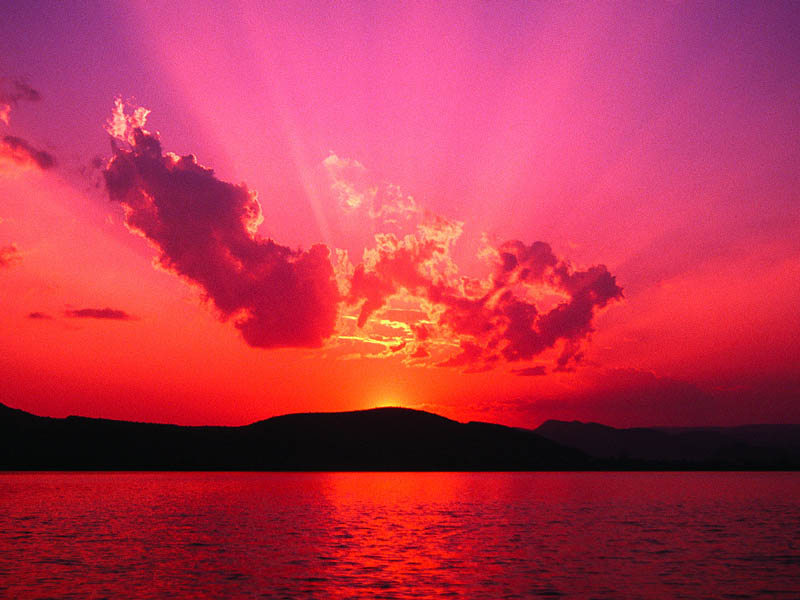
\includegraphics[scale=.50]{Sunset.jpg}
\caption{Sunset figure}
\label{fig:sunset-fig2}
\end{figure}
%%%%%%%%%%%%%%%%%%%%%%%%%%%%%%%%%%%%%%%%%%%%%%%%%%%%%%
\subsubsection{This is a subsubsection}
\begin{table}[H]
\centering
\caption{This is a table template - This is an example of a long table title.  Table titles need to be single-spaced within and double spaced between in the list of tables.}
\begin{tabular}{|l|c|c|c|c|c|}
\hline
Product & 1 & 2 & 3 & 4 & 5\\
\hline
Price & 124.- & 136.- & 85.- & 156.- & 23.-\\
Guarantee [years] & 1 & 2 & - & 3 & 1\\
Rating & 89\% & 84\% & 51\% & & 45\%\\
\hline
\hline
Recommended & yes & yes & no & no & no\\
\hline
\end{tabular}
\label{tab:template1-2}
\end{table}
\section{Another Section}
%%%%%%%%%%%%%%%%%%%%%%%%%%%%%%%%%%%%%%%%%%%%%%%%%%%
%
%  New template code for TAMU Theses and Dissertations starting Fall 2012.  
%  For more info about this template or the 
%  TAMU LaTeX User's Group, see http://www.howdy.me/.
%
%  Author: Wendy Lynn Turner 
%	 Version 1.0 
%  Last updated 8/5/2012
%
%%%%%%%%%%%%%%%%%%%%%%%%%%%%%%%%%%%%%%%%%%%%%%%%%%%
%%%%%%%%%%%%%%%%%%%%%%%%%%%%%%%%%%%%%%%%%%%%%%%%%%%%%%%%%%%%%%%%%%%%%%
%%                           SECTION III
%%%%%%%%%%%%%%%%%%%%%%%%%%%%%%%%%%%%%%%%%%%%%%%%%%%%%%%%%%%%%%%%%%%%%



\chapter{\uppercase{Last Chapter: The Importance of Research}}

Text goes here \cite{Agrawal1986}.

\section{New Section}

%%%%%%%%%%%%%%%%%%%%%%%%%%%%%%%%%%%%%%%%%%%%%%%%%%%%%%
\begin{figure}[H]
\centering
\includegraphics[scale=.50]{Penguins.jpg}
\caption{TAMU figure}
\label{fig:tamu-fig3}
\end{figure}
%%%%%%%%%%%%%%%%%%%%%%%%%%%%%%%%%%%%%%%%%%%%%%%%%%%%%%
\section{Another Section}

Text between the figures.  Text between the figures. Text between the figures. Text between the figures.  Text between the figures. Text between the figures. Text between the figures.  Text between the figures. Text between the figures. Text between the figures.  Text between the figures. Text between the figures.
%%%%%%%%%%%%%%%%%%%%%%%%%%%%%%%%%%%%%%%%%%%%%%%%%%%%%%%
%\begin{figure}[H]
%\centering
%\includegraphics[scale=.50]{figures/Penguins.jpg}
%\caption{Another TAMU figure}
%\label{fig:tamu-fig4}
%\end{figure}
%%%%%%%%%%%%%%%%%%%%%%%%%%%%%%%%%%%%%%%%%%%%%%%%%%%%%%%

\subsection{Subsection}

%%%%%%%%%%%%%%%%%%%%%%%%%%%%%%%%%%%%%%%%%%%%%%%%%%%%%%%
%\begin{figure}[H]
%\centering
%\includegraphics[scale=.50]{figures/Penguins.jpg}
%\caption{Another TAMU figure}
%\label{fig:tamu-fig4-2}
%\end{figure}
%%%%%%%%%%%%%%%%%%%%%%%%%%%%%%%%%%%%%%%%%%%%%%%%%%%%%%%
\subsection{Subsection}

A table example is going to follow.

\begin{table}[H]
\centering
\caption{This is a table template}
\begin{tabular}{|l|c|c|c|c|c|}
\hline
Product & 1 & 2 & 3 & 4 & 5\\
\hline
Price & 124.- & 136.- & 85.- & 156.- & 23.-\\
Guarantee [years] & 1 & 2 & - & 3 & 1\\
Rating & 89\% & 84\% & 51\% & & 45\%\\
\hline
\hline
Recommended & yes & yes & no & no & no\\
\hline
\end{tabular}
\label{tab:template2}
\end{table}
\subsubsection{This is a subsubsection}
\section{Another Section}

fix spacing in bibliography, if any...
%%%%%%%%%%%%%%%%%%%%%%%%%%%%%%%%%%%%%%%%%%%%%%%%%%%%%%%%%%%%%
\let\oldbibitem\bibitem
\renewcommand{\bibitem}{\setlength{\itemsep}{0pt}\oldbibitem}
%%%%%%%%%%%%%%%%%%%%%%%%%%%%%%%%%%%%%%%%%%%%%%%%%%%%%%%%%%%%%%%
%%%%%%%%%%%%%%%%%%%%%%%%%%%%%%%%%%%%%%%%%%%%%%%%%%%
%
%  New template code for TAMU Theses and Dissertations starting Fall 2012.  
%  For more info about this template or the 
%  TAMU LaTeX User's Group, see http://www.howdy.me/.
%
%  Author: Wendy Lynn Turner 
%	 Version 1.0 
%  Last updated 8/5/2012
%
%%%%%%%%%%%%%%%%%%%%%%%%%%%%%%%%%%%%%%%%%%%%%%%%%%%


%%%%%%%%%%%%%%%%%%%%%%%%%%%%%%%%%%%%%%%%%%%%%%%%%%%%%%%%%%%%%%%%%%%%%%
%%                           REFERENCES 
%%%%%%%%%%%%%%%%%%%%%%%%%%%%%%%%%%%%%%%%%%%%%%%%%%%%%%%%%%%%%%%%%%%%%

\phantomsection
\addcontentsline{toc}{chapter}{REFERENCES}

\renewcommand{\bibname}{{\normalsize\rm REFERENCES}}

\bibliographystyle{unsrt}
\bibliography{Mendeley}

% %%%%%%%%%%%%%%%%%%%%%%%%%%%%%%%%%%%%%%%%%%%%%%%%%%%
%
%  New template code for TAMU Theses and Dissertations starting Fall 2012.  
%  For more info about this template or the 
%  TAMU LaTeX User's Group, see http://www.howdy.me/.
%
%  Author: Wendy Lynn Turner 
%	 Version 1.0 
%  Last updated 8/5/2012
%
%%%%%%%%%%%%%%%%%%%%%%%%%%%%%%%%%%%%%%%%%%%%%%%%%%%

\begin{appendices}
\titleformat{\chapter}{\centering\normalsize}{APPENDIX \thechapter}{0em}{\vskip .5\baselineskip\centering}
\renewcommand{\appendixname}{APPENDIX}

%%%%%%%%%%%%%%%%%%%%%%%%%%%%%%%%%%%%%%%%%%%%%%%%%%%
%
%  New template code for TAMU Theses and Dissertations starting Fall 2012.  
%  For more info about this template or the 
%  TAMU LaTeX User's Group, see http://www.howdy.me/.
%
%  Author: Wendy Lynn Turner 
%	 Version 1.0 
%  Last updated 8/5/2012
%
%%%%%%%%%%%%%%%%%%%%%%%%%%%%%%%%%%%%%%%%%%%%%%%%%%%

%%%%%%%%%%%%%%%%%%%%%%%%%%%%%%%%%%%%%%%%%%%%%%%%%%%%%%%%%%%%%%%%%%%%%%
%%                           APPENDIX A 
%%%%%%%%%%%%%%%%%%%%%%%%%%%%%%%%%%%%%%%%%%%%%%%%%%%%%%%%%%%%%%%%%%%%%

\phantomsection

\chapter{\texorpdfstring{\MakeUppercase{Approximations to the Ramp Function}}{Approximations to the Ramp Function}}

\section{Approximation Using Fourier Series}

This section shows a derivation of the Fourier Series for the ramp
function, which is often used to model the output flow for a terminal
unit.

In many cases related to steady state algorithms for determining the
energy use of an air handling unit, ramp functions are found. These ramp
functions are usually difficult to deal with in optimization problems
because they are not continuously differentiable. In this sense, it is
desired to have a replacement or approximation to the function that is
smooth and can be differentiated. 

Fourier series are a useful tool for approximating arbitrary functions
and can be used in this task. We can begin by focusing on the basic ramp
function that is defined by:

\begin{equation}
f(x)=\begin{cases}0  & x < 0 \\
               x  & x \geq 0
\end{cases}
\end{equation}

If we define our Fourier series to be defined over the interval \(-L
\leq x \leq L\) and be equal to 

\begin{equation}
 f(x) = a_0 + \sum_{n=1}^\infty a_n \cos{\frac{n \pi x }{L}} + \sum_{n=1}^\infty b_n \sin{\frac{n \pi x }{L}}
\end{equation}

The coefficients are equal to

\begin{equation}
 a_0 = \frac{1}{2 L } \int_{-L}^{L} f(x) \; dx 
\end{equation}


\begin{equation}
 a_n = \frac{1}{L} \int_{-L}^{L} f(x) \cos{\frac{n \pi x}{L}} \; dx 
\end{equation}

\begin{equation}
 b_n = \frac{1}{L} \int_{-L}^{L} f(x) \sin{\frac{n \pi x}{L}} \; dx 
\end{equation}

\(f(x)=0\) when \(x \leq 0\), so that portion of the integral is equal to 0. When \(x \geq 0\), \(f(x)=x\) and the coefficients can be evaluated over the range \(0 \leq x \leq L\).

\begin{equation}
 a_0 = \frac{1}{2 L } \int_{0}^{L} x \; dx 
\end{equation}


\begin{equation}
 a_n = \frac{1}{L} \int_{0}^{L} x \cos{\frac{n \pi x}{L}} \; dx 
\end{equation}

\begin{equation}
 b_n = \frac{1}{L} \int_{0}^{L} x \sin{\frac{n \pi x}{L}} \; dx 
\end{equation}


Solving for \(a_0\), 
%
\begin{equation}
 a_0 = \frac{1}{2 L } \int_{0}^{L} x \; dx = \frac{1}{2 L} \left[ \frac{x^2}{2} \right]^{L}_{0} = \frac{1}{2 L} \left(\frac{L^2}{2} \right) = \frac{L}{4}
\end{equation}
%
The coefficients for the cosine terms are 
%
\begin{equation}
 \begin{split} 
     a_n &= \frac{1}{L} \int_{0}^{L} x \cos{\frac{n \pi x}{L}} \; dx \\ 
         &=  \frac{1}{L} \left(\cancelto{0}{x \frac{L}{n \pi}   \sin{\frac{n \pi x}{L}}  \bigg|^{L}_0}  - \int_0^L \frac{L}{n \pi} \sin{\frac{n \pi}{L} x} \; dx  \right) \\
         &= \frac{1}{L} \left( \left[ \frac{L^2}{n^2 \pi^2} \cos{\frac{n \pi x}{L}}  \right]^L_0 \right) \\
         &= \frac{L}{n^2 \pi^2}\left( (-1)^n - 1 \right)
 \end{split}
\end{equation}
%
%
and the coefficients for the sine terms are 
%
%
\begin{equation}
 \begin{split} 
     b_n &= \frac{1}{L} \int_{0}^{L} x \sin{\frac{n \pi x}{L}} \; dx \\ 
         &=  \frac{1}{L} \left(-x \frac{L}{n \pi}   \cos{\frac{n \pi x}{L}}  \bigg|^{L}_0  - \int_0^L -\frac{L}{n \pi}\cos{\frac{n \pi}{L} x} \; dx  \right) \\
         &= \frac{1}{L} \left( \left[ \frac{-L^2}{n \pi} (-1)^n  +\frac{L^2}{n^2 \pi^2}   \left[ \sin{\frac{n \pi x}{L}} \right]_0^L  \right] \right) \\
         &= \frac{1}{L} \left( \left[ \frac{-L^2}{n \pi} (-1)^n  + 0 \right] \right) \\
         &= \frac{L}{n \pi}\left( (-1)^{n+1} \right)
 \end{split}
\end{equation}
%\begin{figure}[H]
%\centering
%\includegraphics[scale=.50]{figures/Penguins.jpg}
%\caption{TAMU figure}
%\label{fig:tamu-fig5}
%\end{figure}

\section{Approximation Using the Logistic Function}

The threshold function is the derivative of the ramp function. The
threshold function can be approximated arbitrarily well using the
logistic function. The logistic function has the form
\begin{equation}\label{eq:ThresholdFunction}
    y=\frac{1}{1+e^{-k\left(x-x_{0}\right)}}  
\end{equation}
As \(k\to\infty\), the function equals the threshold function. The
integral of the threshold function is the ramp function. Integrating 
Eq. \ref{eq:ThresholdFunction} results in 
\begin{equation}
    y=\frac{\ln \left(1+e^{k\left(x-x_{0}\right)}\right) }{k} + C
\end{equation}
This function approximates the ramp function arbitrarily well as
\(k\to\infty\). 

The function is usually applied to flow for terminal units with a
minimum flow setting. In this case, the function becomes

\begin{equation}
    \flow{} = \frac{\ln{} \left(1+e^{k\left( \flow{req} - \flow{min} \right)}\right)}{k} + \flow{min}
\end{equation}



%%%%%%%%%%%%%%%%%%%%%%%%%%%%%%%%%%%%%%%%%%%%%%%%%%%
%
%  New template code for TAMU Theses and Dissertations starting Fall 2012.  
%  For more info about this template or the 
%  TAMU LaTeX User's Group, see http://www.howdy.me/.
%
%  Author: Wendy Lynn Turner 
%	 Version 1.0 
%  Last updated 8/5/2012
%
%%%%%%%%%%%%%%%%%%%%%%%%%%%%%%%%%%%%%%%%%%%%%%%%%%%

%%%%%%%%%%%%%%%%%%%%%%%%%%%%%%%%%%%%%%%%%%%%%%%%%%%%%%%%%%%%%%%%%%%%%%
%%                           APPENDIX B
%%%%%%%%%%%%%%%%%%%%%%%%%%%%%%%%%%%%%%%%%%%%%%%%%%%%%%%%%%%%%%%%%%%%%

\chapter{\texorpdfstring{\MakeUppercase{ZONE LOADS FOR NCTM}}{Zone Loads
for NCTM}}

\section{Estimated Zone Loads for NCTM}

This portion of the appendix plots all the zone loads for the terminal
units at NCTM. 

\newcommand{\zoneLoadAppendixPlotsCaption}[1]{Zone load for #1 during
the year 2016.}

\section{Terminal Units of AHU-2-1}
%Plots/04/2017-06-27-0830-BtuhrvsOADryBulbTemperatureNOAAF.tex
\begin{figure}
    \centering
    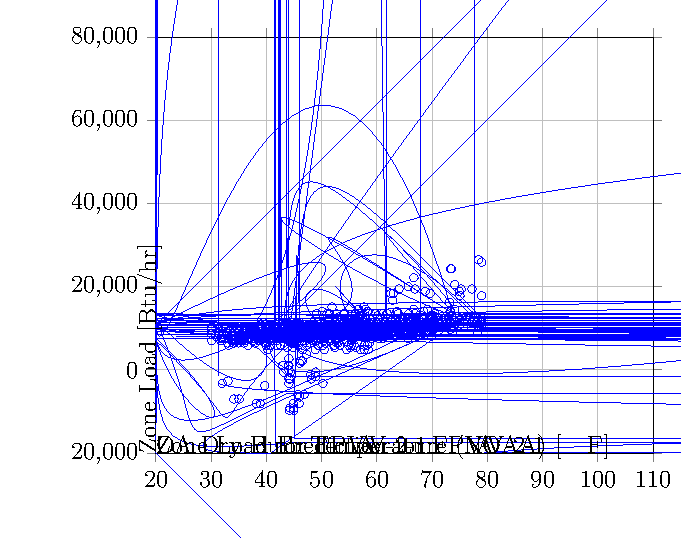
\includegraphics{Plots/04/2017-06-27-0830-BtuhrvsOADryBulbTemperatureNOAAF.pdf}
    \caption{\zoneLoadAppendixPlotsCaption{FPVAV-2-1}}
    \label{fig:2017-06-27-0830-BtuhrvsOADryBulbTemperatureNOAAF}
\end{figure}

\begin{figure}
    \centering
    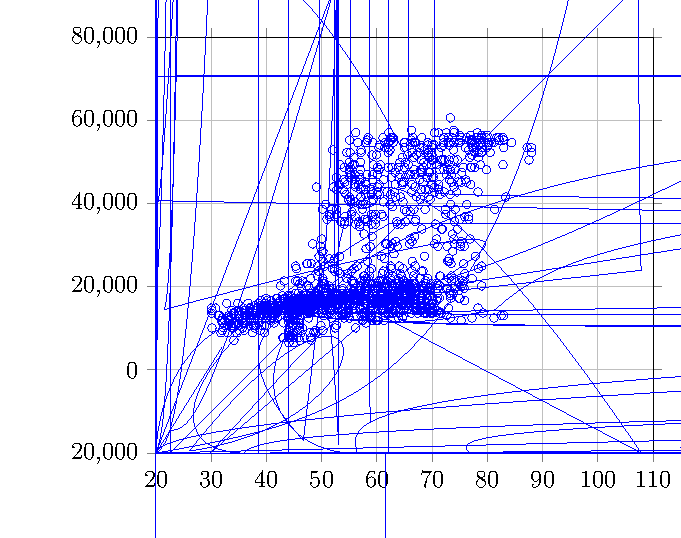
\includegraphics{Plots/05/2017-06-27-1012-BtuhrvsOADryBulbTemperatureNOAAF.pdf}
    \caption{\zoneLoadAppendixPlotsCaption{FPVAV-2-2}}
    \label{fig:2017-06-27-1012-BtuhrvsOADryBulbTemperatureNOAAF}
\end{figure}

\begin{figure}
\centering
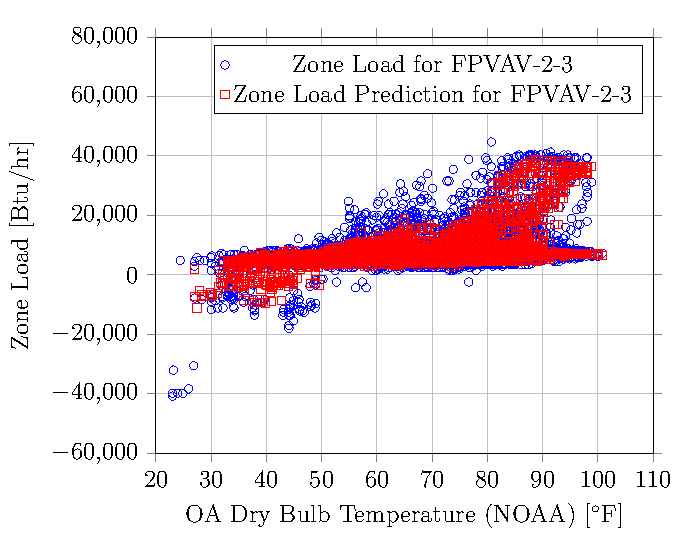
\includegraphics{Plots/06/2017-06-27-1018-BtuhrvsOADryBulbTemperatureNOAAF.pdf}
\caption{\zoneLoadAppendixPlotsCaption{FPVAV-2-3} Notice that the lower
bound of the y-axis is different than the other plots. }
\label{fig:2017-06-27-1018-BtuhrvsOADryBulbTemperatureNOAAF}
\end{figure}


\clearpage

\section{Terminal Units of AHU-2-2}

\begin{figure}
\centering
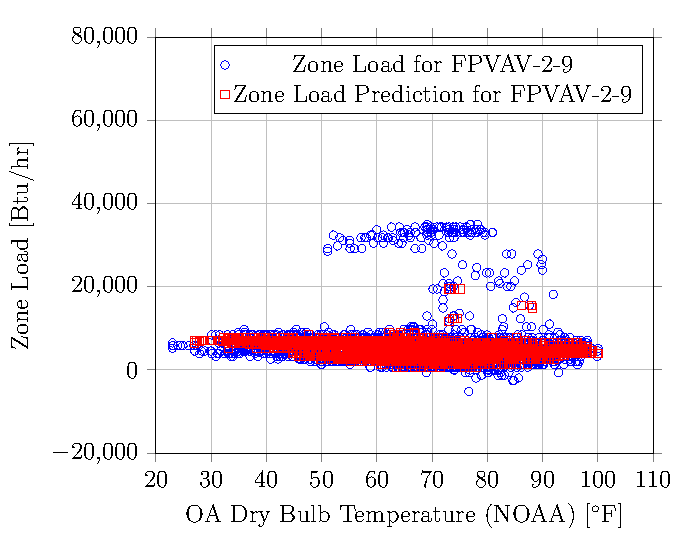
\includegraphics{Plots/07/2017-06-27-1026-BtuhrvsOADryBulbTemperatureNOAAF.pdf}
\caption{\zoneLoadAppendixPlotsCaption{FPVAV-2-9}}
\label{fig:2017-06-27-1026-BtuhrvsOADryBulbTemperatureNOAAF}
\end{figure}

\begin{figure}
\centering
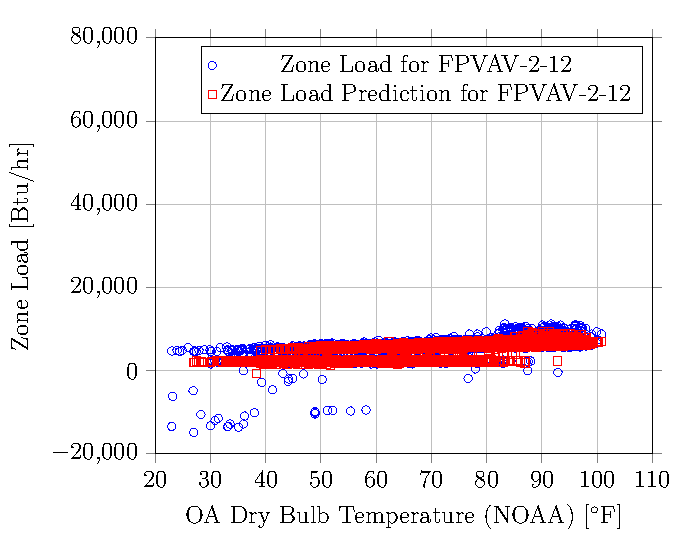
\includegraphics{Plots/08/2017-06-27-1058-BtuhrvsOADryBulbTemperatureNOAAF.pdf}
\caption{\zoneLoadAppendixPlotsCaption{FPVAV-2-12}}
\label{fig:2017-06-27-1058-BtuhrvsOADryBulbTemperatureNOAAF}
\end{figure}


\begin{figure}
\centering
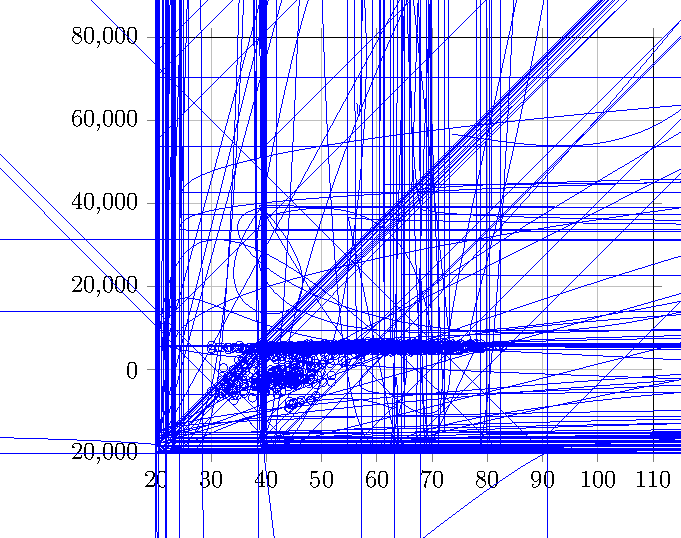
\includegraphics{Plots/09/2017-06-27-1124-BtuhrvsOADryBulbTemperatureNOAAF.pdf}
\caption{\zoneLoadAppendixPlotsCaption{FPVAV-2-13}}
\label{fig:2017-06-27-1124-BtuhrvsOADryBulbTemperatureNOAAF}
\end{figure}

\begin{figure}
\centering
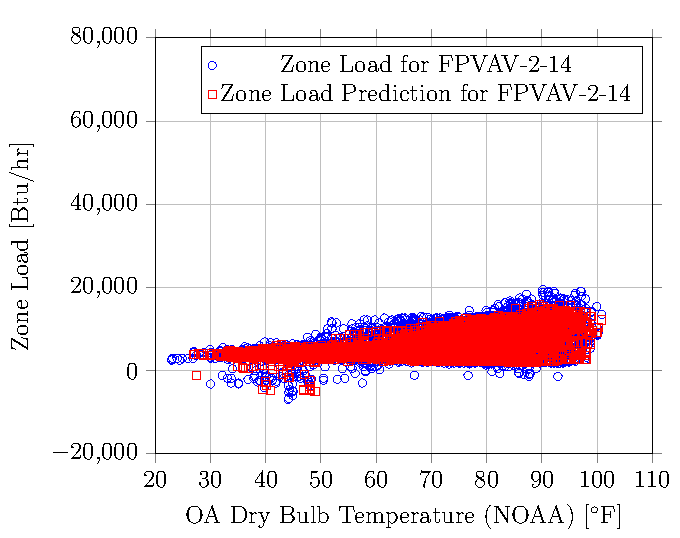
\includegraphics{Plots/10/2017-06-27-1131-BtuhrvsOADryBulbTemperatureNOAAF.pdf}
\caption{\zoneLoadAppendixPlotsCaption{FPVAV-2-14}}
\label{fig:2017-06-27-1131-BtuhrvsOADryBulbTemperatureNOAAF}
\end{figure}

\begin{figure}
\centering
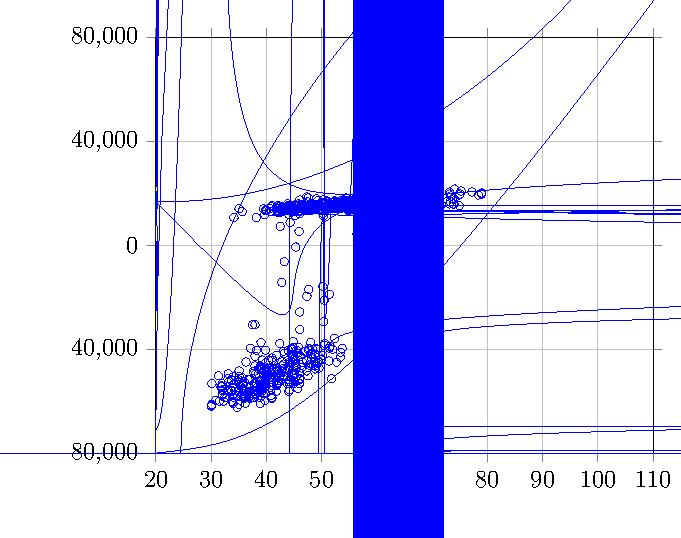
\includegraphics{Plots/11/2017-06-27-1135-BtuhrvsOADryBulbTemperatureNOAAF.pdf}
\caption{\zoneLoadAppendixPlotsCaption{FPVAV-2-15} Notice that the lower
bound of the y-axis is different than the other plots.}
\label{fig:2017-06-27-1135-BtuhrvsOADryBulbTemperatureNOAAF}
\end{figure}

\begin{figure}
\centering
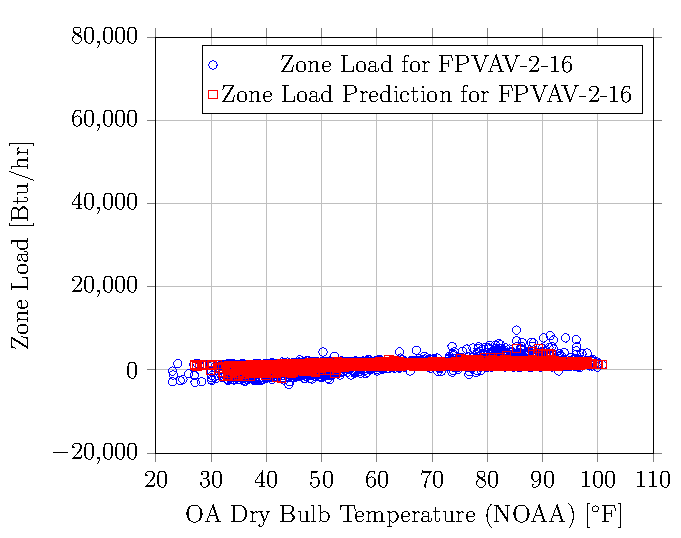
\includegraphics{Plots/12/2017-06-27-1138-BtuhrvsOADryBulbTemperatureNOAAF.pdf}
\caption{\zoneLoadAppendixPlotsCaption{FPVAV-2-16}}
\label{fig:2017-06-27-1138-BtuhrvsOADryBulbTemperatureNOAAF}
\end{figure}


\begin{figure}
    \centering
    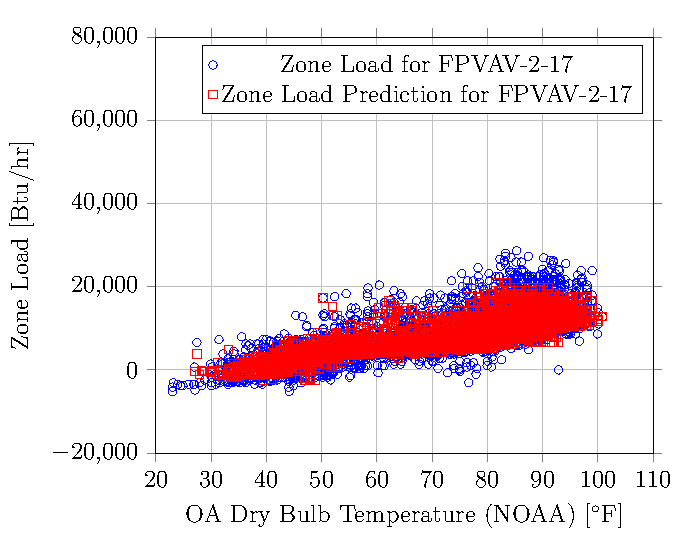
\includegraphics{Plots/13/2017-06-27-1141-BtuhrvsOADryBulbTemperatureNOAAF.pdf}
    \caption{\zoneLoadAppendixPlotsCaption{FPVAV-2-17}}
    \label{fig:2017-06-27-1141-BtuhrvsOADryBulbTemperatureNOAAF}
\end{figure}

\begin{figure}
\centering
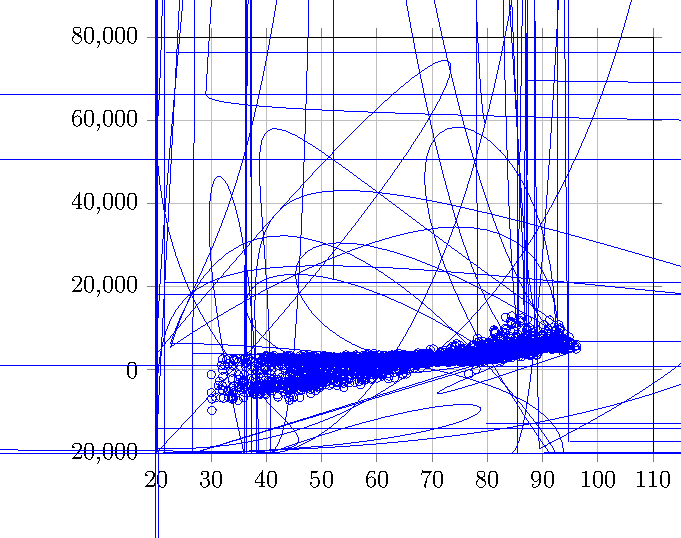
\includegraphics{Plots/14/2017-06-27-1145-BtuhrvsOADryBulbTemperatureNOAAF.pdf}
\caption{\zoneLoadAppendixPlotsCaption{FPVAV-2-18}}
\label{fig:2017-06-27-1145-BtuhrvsOADryBulbTemperatureNOAAF}
\end{figure}


\section{Terminal Units of AHU-2-3}

\begin{figure}
\centering
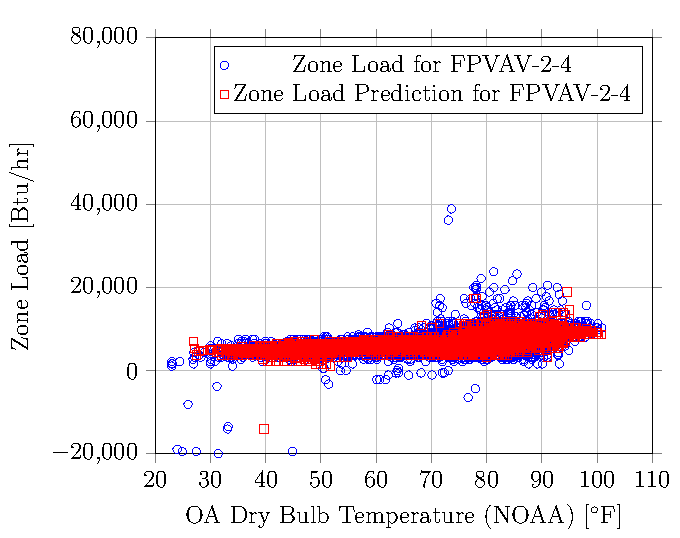
\includegraphics[]{Plots/15/2017-06-27-1319-BtuhrvsOADryBulbTemperatureNOAAF.pdf}
\caption{\zoneLoadAppendixPlotsCaption{FPVAV-2-4}}
\label{fig:2017-06-27-1319-BtuhrvsOADryBulbTemperatureNOAAF}
\end{figure}

\begin{figure}
\centering
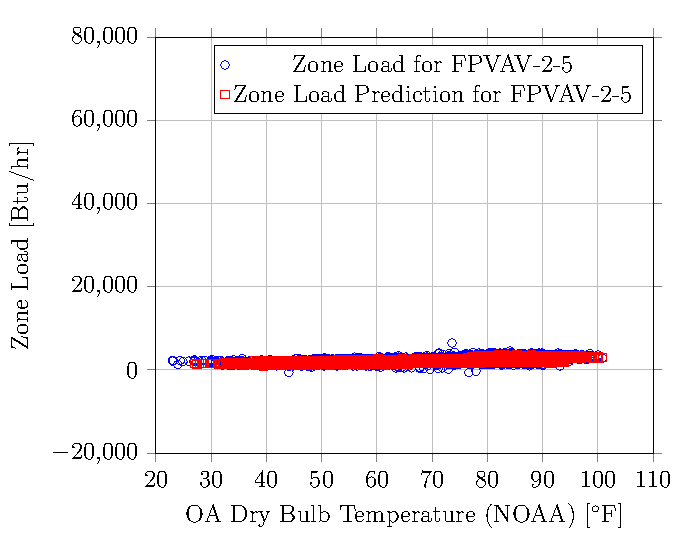
\includegraphics[]{Plots/16/2017-06-27-1322-BtuhrvsOADryBulbTemperatureNOAAF.pdf}
\caption{\zoneLoadAppendixPlotsCaption{FPVAV-2-5}}
\label{fig:2017-06-27-1322-BtuhrvsOADryBulbTemperatureNOAAF}
\end{figure}

\begin{figure}
\centering
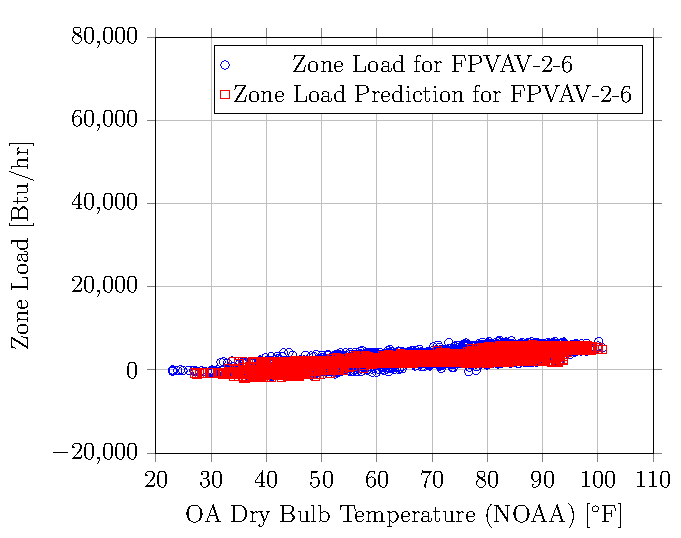
\includegraphics[]{Plots/17/2017-06-27-1325-BtuhrvsOADryBulbTemperatureNOAAF.pdf}
\caption{\zoneLoadAppendixPlotsCaption{FPVAV-2-6}}
\label{fig:2017-06-27-1325-BtuhrvsOADryBulbTemperatureNOAAF}
\end{figure}


\begin{figure}
\centering
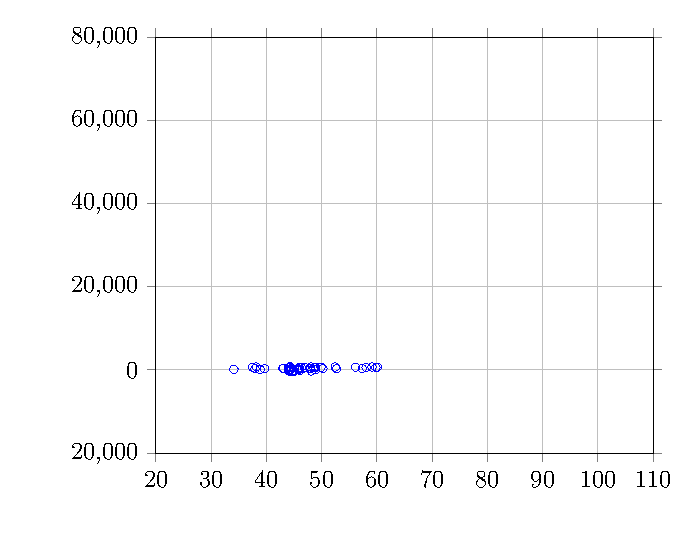
\includegraphics[]{Plots/18/2017-06-27-1328-BtuhrvsOADryBulbTemperatureNOAAF.pdf}
\caption{\zoneLoadAppendixPlotsCaption{FPVAV-2-7}}
\label{fig:2017-06-27-1328-BtuhrvsOADryBulbTemperatureNOAAF}
\end{figure}

\begin{figure}
\centering
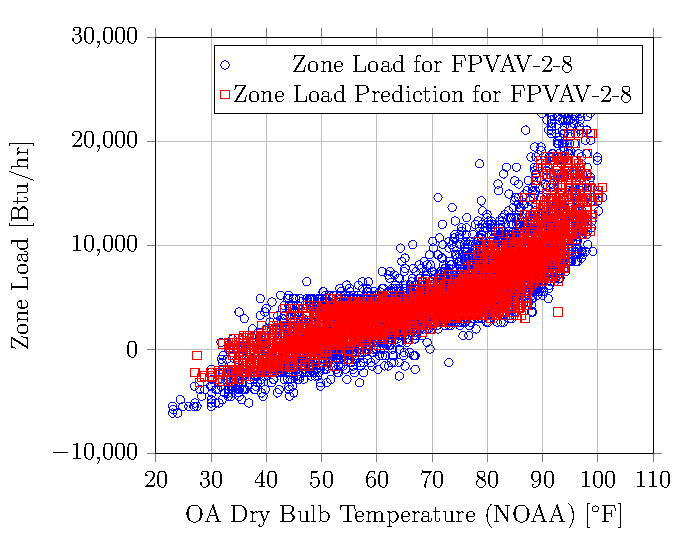
\includegraphics[]{Plots/19/2017-06-27-1330-BtuhrvsOADryBulbTemperatureNOAAF.pdf}
\caption{\zoneLoadAppendixPlotsCaption{FPVAV-2-8}}
\label{fig:2017-06-27-1330-BtuhrvsOADryBulbTemperatureNOAAF}
\end{figure}

\begin{figure}
\centering
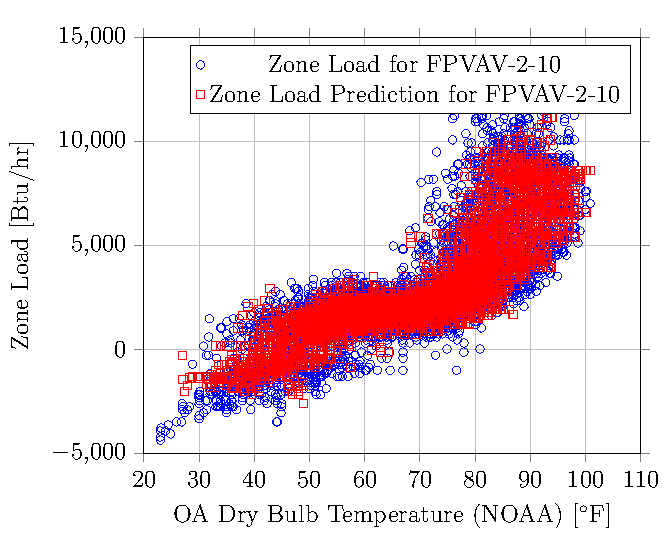
\includegraphics[]{Plots/20/2017-06-27-1332-BtuhrvsOADryBulbTemperatureNOAAF.pdf}
\caption{\zoneLoadAppendixPlotsCaption{FPVAV-2-10}}
\label{fig:2017-06-27-1332-BtuhrvsOADryBulbTemperatureNOAAF}
\end{figure}

\begin{figure}
\centering
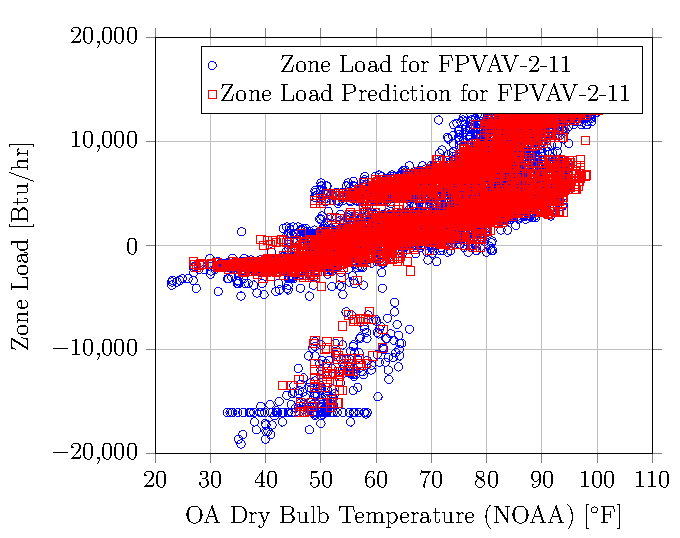
\includegraphics[]{Plots/21/2017-06-27-1334-BtuhrvsOADryBulbTemperatureNOAAF.pdf}
\caption{\zoneLoadAppendixPlotsCaption{FPVAV-2-11}}
\label{fig:2017-06-27-1334-BtuhrvsOADryBulbTemperatureNOAAF}
\end{figure}

\section{Terminal Units of AHU-1-2}

\begin{figure}
    \centering
    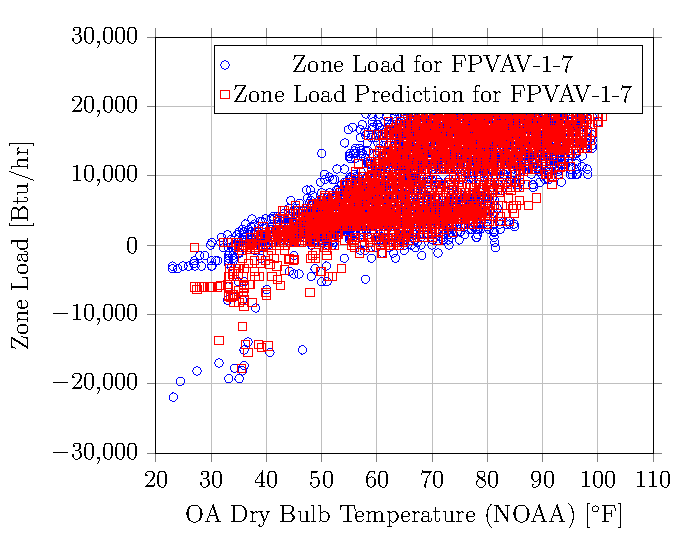
\includegraphics[]{Plots/22/2017-06-27-1343-BtuhrvsOADryBulbTemperatureNOAAF.pdf}
    \caption{\zoneLoadAppendixPlotsCaption{FPVAV-1-7}}
    \label{fig:2017-06-27-1343-BtuhrvsOADryBulbTemperatureNOAAF}
\end{figure}

\begin{figure}
\centering
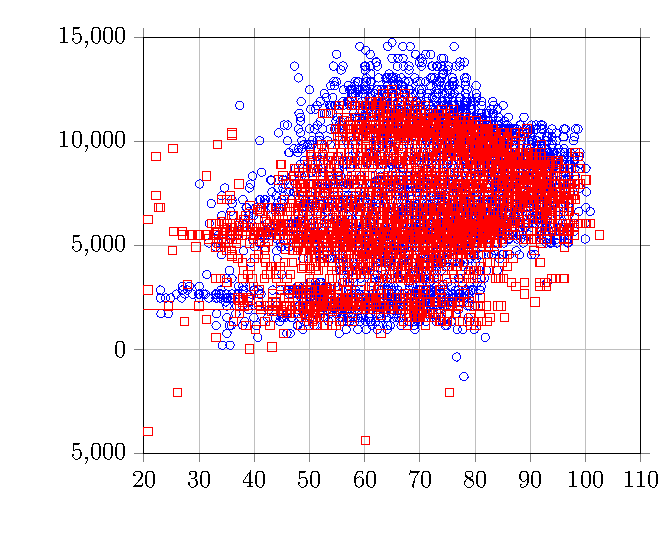
\includegraphics[]{Plots/23/2017-06-27-1346-BtuhrvsOADryBulbTemperatureNOAAF.pdf}
\caption{\zoneLoadAppendixPlotsCaption{FPVAV-1-8}}
\label{fig:2017-06-27-1346-BtuhrvsOADryBulbTemperatureNOAAF}
\end{figure}

\begin{figure}
\centering
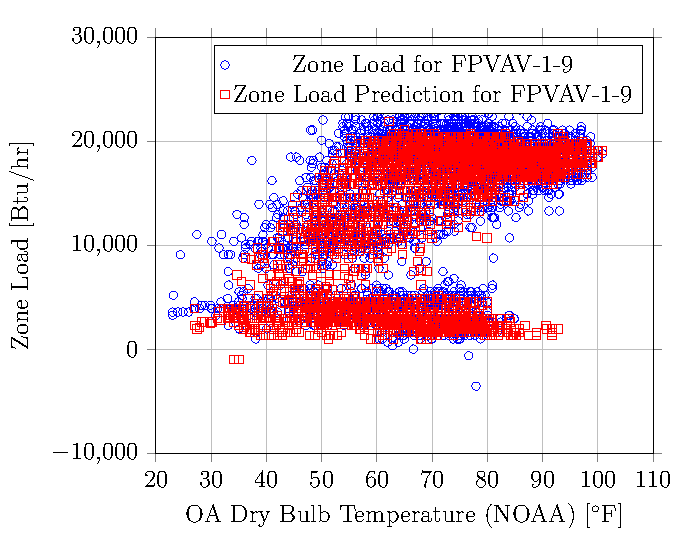
\includegraphics[]{Plots/24/2017-06-27-1348-BtuhrvsOADryBulbTemperatureNOAAF.pdf}
\caption{\zoneLoadAppendixPlotsCaption{FPVAV-1-9}}
\label{fig:2017-06-27-1348-BtuhrvsOADryBulbTemperatureNOAAF}
\end{figure}

\begin{figure}
\centering
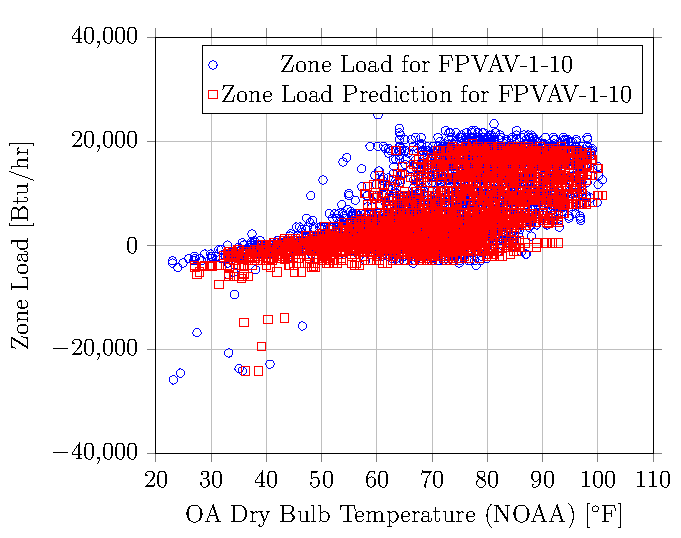
\includegraphics[]{Plots/25/2017-06-27-1353-BtuhrvsOADryBulbTemperatureNOAAF.pdf}
\caption{\zoneLoadAppendixPlotsCaption{FPVAV-1-10}}
\label{fig:2017-06-27-1353-BtuhrvsOADryBulbTemperatureNOAAF}
\end{figure}

\section{Terminal Units of AHU-1-3}

\begin{figure}
\centering
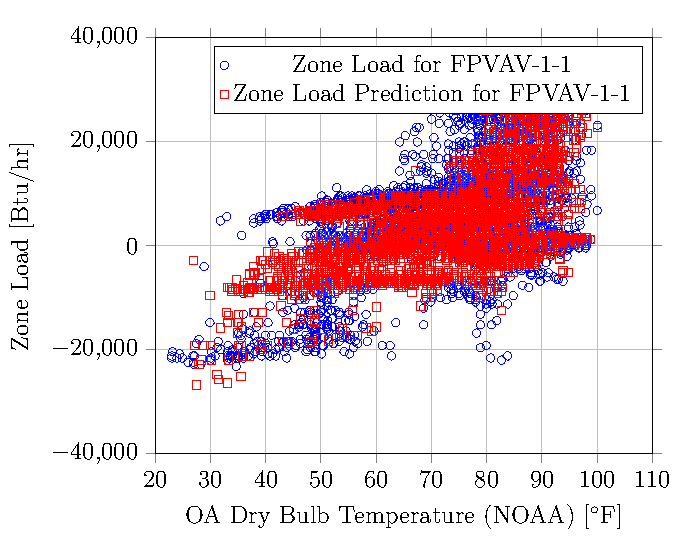
\includegraphics[]{Plots/26/2017-06-27-1355-BtuhrvsOADryBulbTemperatureNOAAF.pdf}
\caption{\zoneLoadAppendixPlotsCaption{FPVAV-1-1}}
\label{fig:2017-06-27-1355-BtuhrvsOADryBulbTemperatureNOAAF}
\end{figure}

\begin{figure}
\centering
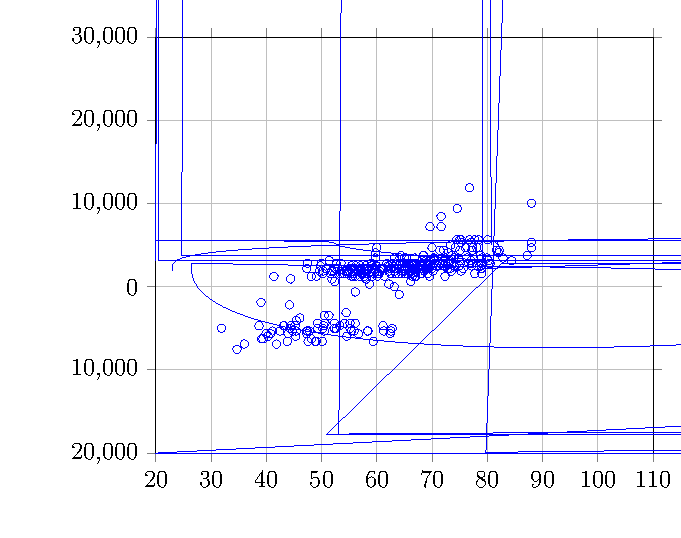
\includegraphics[]{Plots/27/2017-06-27-1356-BtuhrvsOADryBulbTemperatureNOAAF.pdf}
\caption{\zoneLoadAppendixPlotsCaption{FPVAV-1-2}}
\label{fig:2017-06-27-1356-BtuhrvsOADryBulbTemperatureNOAAF}
\end{figure}

\begin{figure}
\centering
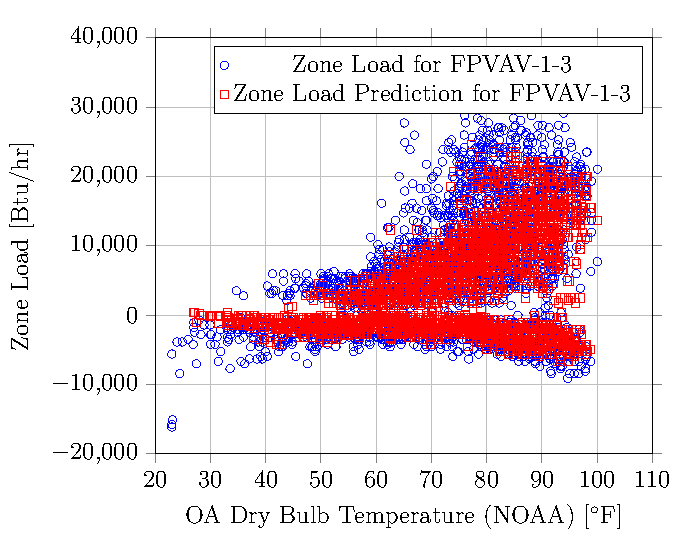
\includegraphics[]{Plots/28/2017-06-27-1357-BtuhrvsOADryBulbTemperatureNOAAF.pdf}
\caption{\zoneLoadAppendixPlotsCaption{FPVAV-1-3}}
\label{fig:2017-06-27-1357-BtuhrvsOADryBulbTemperatureNOAAF}
\end{figure}

\begin{figure}
\centering
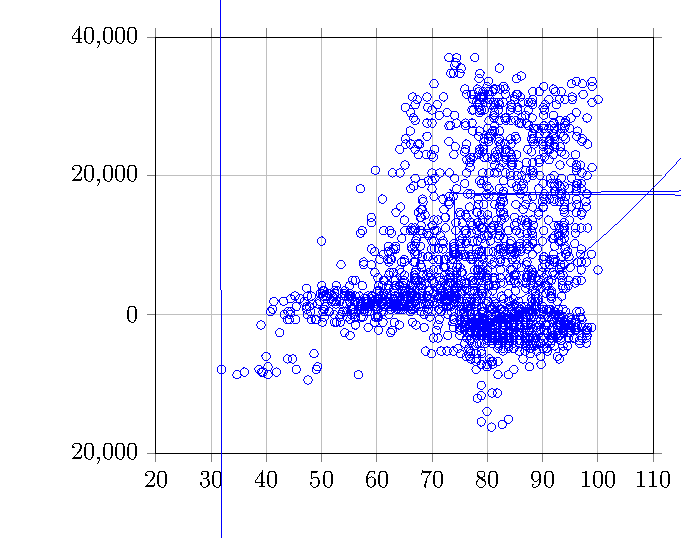
\includegraphics[]{Plots/29/2017-06-27-1358-BtuhrvsOADryBulbTemperatureNOAAF.pdf}
\caption{\zoneLoadAppendixPlotsCaption{FPVAV-1-4}}
\label{fig:2017-06-27-1358-BtuhrvsOADryBulbTemperatureNOAAF}
\end{figure}

\begin{figure}
\centering
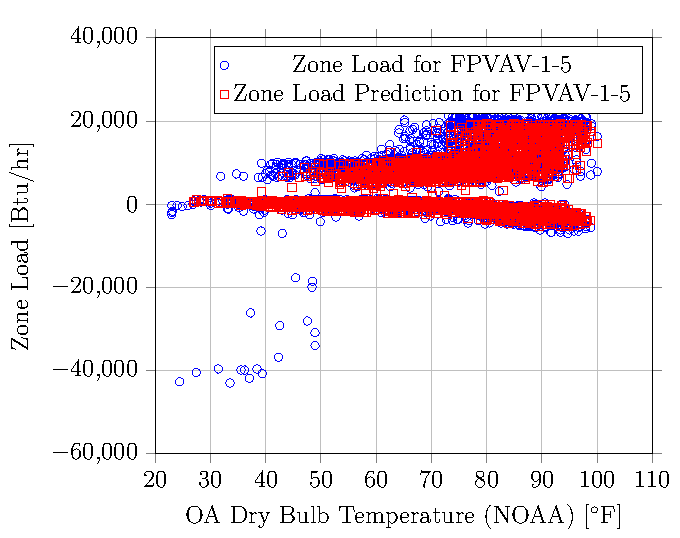
\includegraphics[]{Plots/30/2017-06-27-1359-BtuhrvsOADryBulbTemperatureNOAAF.pdf}
\caption{\zoneLoadAppendixPlotsCaption{FPVAV-1-5}}
\label{fig:2017-06-27-1359-BtuhrvsOADryBulbTemperatureNOAAF}
\end{figure}

\begin{figure}
\centering
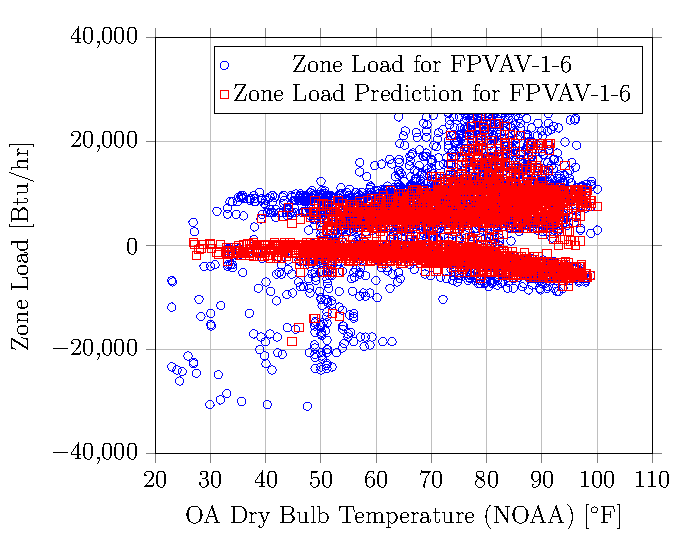
\includegraphics[]{Plots/31/2017-06-27-1400-BtuhrvsOADryBulbTemperatureNOAAF.pdf}
\caption{\zoneLoadAppendixPlotsCaption{FPVAV-1-6}}
\label{fig:2017-06-27-1401-BtuhrvsOADryBulbTemperatureNOAAF}
\end{figure}




\pagebreak{}


\end{appendices}



\end{document}
